\section{Related Work}
In this section, we briefly review some existing neural matching models and graph neural networks.

\subsection{Neural Matching Models}
Most neural matching models fall within two categories: representation-focused models, e.g. DSSM \cite{huang2013learning}, ARC-I \cite{hu2014convolutional}, CDSSM \cite{shen2014latent}, and interaction-focused models, e.g. MatchPyramid \cite{pang2016text}, DRMM \cite{guo2016deep}, PACRR \cite{hui2017pacrr}, KNRM \cite{xiong2017end}.

The representation-focused models follow the representation learning approach adopted in many natural language processing tasks. Queries and documents are projected into the same semantic space individually. The cosine similarity is then used between their high-level text representations to produce the final relevance score. For example, DSSM \cite{huang2013learning}, one of the earliest neural relevance matching models, employs simple dense neural layers to learn high-level representations for queries and documents. To enhance the projecting function, ARC-I \cite{hu2014convolutional} and CDSSM \cite{shen2014latent} devoted much effort into convolutional layers later on. 

In comparison, interaction-focused methods model the two text sequences jointly, by directly exploiting detailed query-document interaction signals rather than high-level representations of individual texts. For example, DRMM \cite{guo2016deep} maps the local query-document interaction signals into a fixed-length histogram, and dense neural layers are followed to produce final ranking scores. \citet{xiong2017end} and \citet{dai2018convolutional} both use kernel pooling to extract multi-level soft match features. Many other works rely on convolutional layers or spatial GRU over interaction signals to extract ranking features  
such as \cite{pang2016text,pang2017deeprank,hui2017pacrr,hui2018co,fan2018modeling}, which considers just local word connections. 

There are also several studies investigating how to apply BERT in ranking, e.g.  \citet{dai2019deeper} and \citet{macavaney2019cedr}. A common approach is to concatenate the document and query text together and feed them into the next sentence prediction task, where the `[CLS]' token embeds the representation of the query-document pair. 
\begin{figure*}[h]
	\centering
	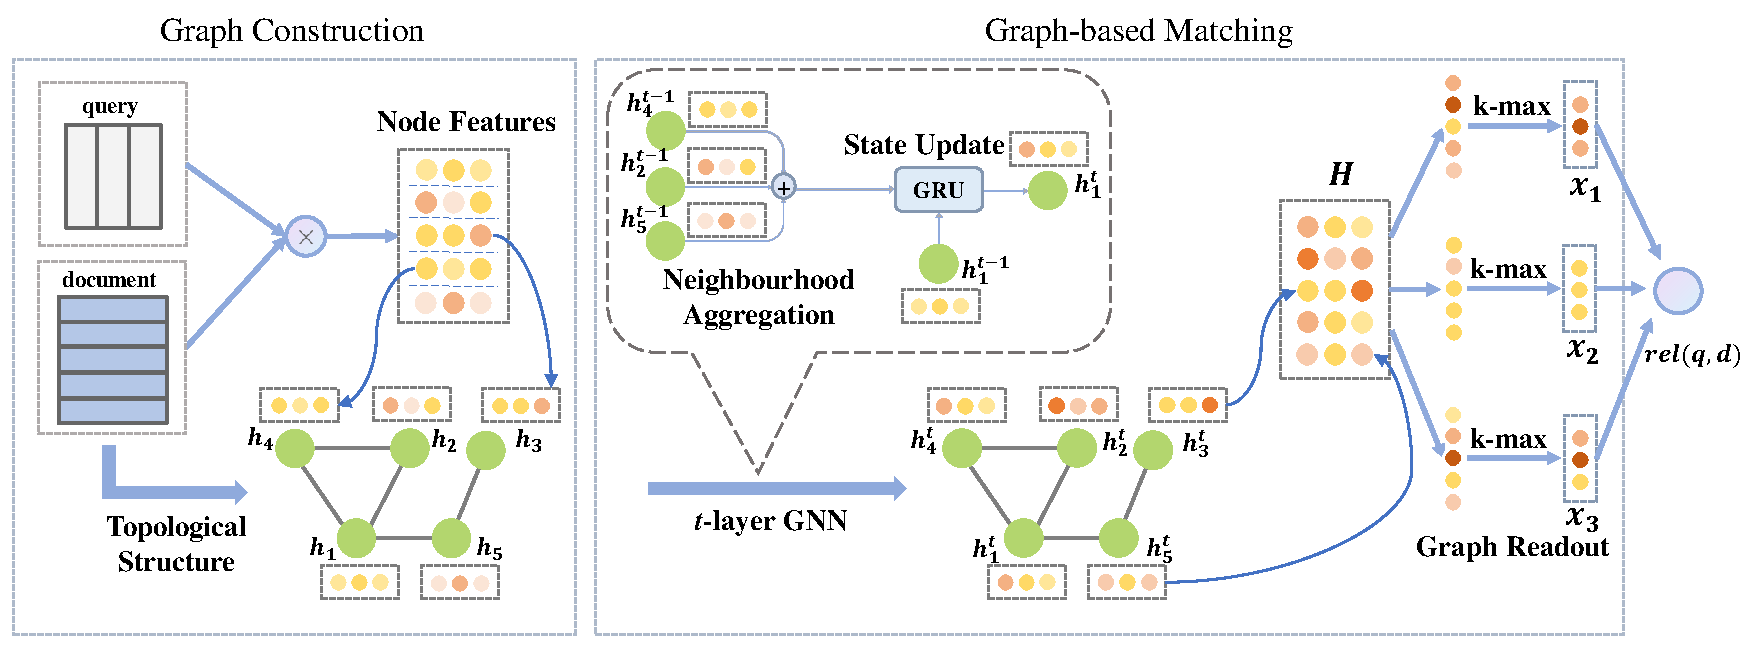
\includegraphics[width=\textwidth]{./pics/grmm.pdf}
	\caption{The workflow of the GRMM model. The document is first transformed into the graph-of-word form, where the node feature is the similarity between the word and each query term. Then, graph neural networks are applied to propagate these matching signals on the document graph. Finally, to estimate a relevance score, top-$k$ signals of each query term are chosen to filter out irrelevant noisy information, and their features are fed into a dense neural layer. }
	\label{fig:2} 
\end{figure*}

Nevertheless, the majority of existing neural matching models only take the linear text sequence, inevitably limiting the model capability. To this end, we propose to break the linear text format and represent the document in a flexible graph structure, where comprehensive interactions can be explicitly modeled. 



\subsection{Graph Neural Networks}
Graph is a kind of data structure which cooperates with a set of objects (nodes) and their relationships (edges). Recently, researches of analysing graphs with machine learning have attracted much attention because of its great representative power in many fields. 

Graph neural networks (GNNs) are deep learning based methods that operate in the graph domain. The concept of GNNs is previously proposed by  \cite{scarselli2008graph}. Generally, nodes in GNNs update own hidden states by aggregating neighbourhood information and mixing things up into a new context-aware state. There are also many variants of GNNs with various kinds of aggregators and updaters, such as \cite{li2016gated,kipf2017semi,hamilton2017inductive,velivckovic2018graph}. 

Due to the convincing performance and high interpretability, GNNs have become a widely applied structural analysis tool. Recently, there are many applications covering from recommendation \cite{wu2019session,li2019fi} to NLP area, including text classification \cite{yao2019graph,zhang2020every}, question answering \cite{de2019question}, and spam review detection \cite{li2019spam}.

In this work, we employ GNNs in the relevance matching task to extract implicit matching patterns from the query-document interaction signals, which is intrinsically difficult to be revealed by existing methods. 

